\chapter{Background and Analysis}
\section{Learning agent}
When we talk about artificial intelligence in games it is often in relation to the concept of an \textit{agent}. In this paper I follow the definition in Stuart Russel and Peter Norvig's book \textit{Artificial Intelligence - A Modern Approach (3rd ed)}. Here an agent is defined as an entity that acts autonomously to stimuli, adapts to changing circumstances, and strives to achieve a goal in a somewhat rational or optimal fashion\cite[4-5,15]{Russell2010}.

The goal of this project is to examine how well an agent can learn playing the game of Hex with an AlphaZero approach, on consumer grade hardware. A very succinct definition of machine learning is from the American computer scientist Tom Mitchell's 1997 book \textit{Machine Learning}:
\begin{displayquote}
A computer  program is  said to learn from experience \textit{E} with respect to  some class of tasks \textit{T} and performance  measure \textit{P}, if its performance at  tasks in \textit{T}, as measured by \textit{P}, improves with experience \textit{E}\cite[2]{Mitchell1997}.
\end{displayquote}

Using the definition above to outline the problem at hand for the learning agents in this project: The task \textit{T} is to play the game of Hex; The performance \textit{P} can be measured by how well they competes against other Hex AI agents, specifically measured by Elo rating; and the training experience \textit{T} consists of former iterations of the models, playing against themselves.

\section{Tree Search}
For some simple games it is perfectly fine to solve them simply by doing a brute force tree search, from the start of the game, and then examine which action paths guarantees a favourably goal state. An example of such a game is Tic-Tac-Toe. For more complex games, a traversal of a tree consisting of all possible action paths through the state space is impractical. For instance, the American mathematician Claude Shannon gave a conservative estimate of the game tree complexity of Chess at 10\textsuperscript{120}, which today is known as the \textit{Shannon number}.

When doing tree traversal of complex games, some sort of heuristic\footnote{A function that guides search.} is often applied, to limit the breadth and depth of the search, and use a value estimation of game states that are not terminal. One problem with this is the \textit{horizon effect} where game states further down the tree, just beyond the "horizon", might lead to a wildly different outcome than the one being evaluated.

Chess has long been the pinnacle of AI research in games. Chess presents a rather difficult task with its game complexity, and enjoys a large degree of popularity around the globe. The first computer chess program to win against a reigning chess world champion, was IBM's Deep Blue, which did so in 1997. An impressive achievement that used all the, at the time, tricks of the trade\footnote{It implemented quiescence search, iterative deepening, transposition tables, NegaScout, an opening book, endgame book, among other things.}. But relative to this thesis' problem, it depended heavily on specialized hardware. Its evaluation functions were also very game specific, based on human chess-playing strategies, which were directly implemented into the hardware\cite{Campbell2002}.

For games with a higher \textit{branching factor}\footnote{The average number of legal moves in a game of average length.} than chess, the tree depth that can be reached in a reasonable time is shallower, compared to Deep Blue, using the same techniques. A game like Go is one of those. Go is commonly played on a 19x19 board, which gives a branching factor of 250 for games of average length, compared to 35 for Chess. For this reason researchers came up with a traversal technique that grows a game tree asymmetrically, but still finds a balance between exploration and exploitation, breadth and depth. This has come to be known as \textit{Monte Carlo tree search} (MCTS). In the original version, evaluation of game states is being done by a approximating a value through random roll-outs to a terminal state. Because of this, MCTS can be said to be of a more general nature, compared to tree search techniques that use domain-specific evaluations. When the number of times a single game tree is traversed goes towards infinity, it is proven, under some conditions, that the algorithm will converge on an optimal action\cite{Coulom2009}. MCTS was successfully applied to the game of Go, but still without acquiring superhuman skill level.

\section{DeepMind's AlphaZero}
Because of the historical primacy of agents with domain-specific heuristics built into their algorithm, it was an astonishing feat when the Alphabet Inc. owned company DeepMind published results of their general purpose reinforcement learning algorithm AlphaZero. This algorithm was able to achieve superhuman game playing skill, starting from tabula rasa, and only training on data generated by self-play\cite{Silver2018}.

AlphaZero is a continuation of DeepMind's Go playing algorithm AlphaGo which gave Deepmind popular fame when it was the first AI agent able to beat a professional Go player of the highest rank, South Korean Lee Sedol, in 2016\cite{Silver2017}. AlphaZero in contrast to AlphaGo is more generic, and results showed that it was able to master several different abstract strategy games: Chess, Shogi, and Go\cite{Silver2018}.

The AlphaZero algorithm uses a single deep Residual Network (ResNet) model, which is initialized with random weights and implemented by the use of the machine learning library Tensorflow. During execution, when the agent is tasked with suggesting a move, it uses a MCTS, to explore a game tree. Here the model is fed game state information translated into an image\footnote{Here an image should be understood as game state features converted into a multi-dimensional binary array.}, to both predict the value of a game state to guide exploitation, and a policy of actions from the game state to guide exploration.

During training of the models, for each of the games Chess, Shogi, and Go, Deepmind used 5,000 1st generation \textit{TPU}s to generate game data. TPU stands for Tensor Processing Unit, and is Google-engineered hardware specialized for neural network machine learning in their server farms, in particular fast matrix multiplication with low energy consumption. It is difficult to find performance information for this specific piece of hardware, but the 2nd generation TPU has a theoretical computational performance of 45 TFLOPS\footnote{FLOPS: Floating Point Operations per second. TFLOPS = 10\textsuperscript{12} FLOPS}\cite{Kennedy2017}. For the game of Chess they spent 9 hours of training and game playing, 12 hours for Shogi, and 13 days for Go on a 19x19 board\cite{Silver2018}. Had they run it on a single TPU, instead of the 5,000, that would have amounted to $\approx 5$, $\approx 7$, and $\approx 178$ years respectively.

\section{Consumer grade hardware}
In many parts of machine learning, and deep learning in particular, normal Central Processing Units (CPU) do not suffice. What is needed is hardware that is capable of loading large quantities of data fast, getting access to said data quickly, and perform many operations in parallel. For this reason a Graphical Processing Unit (GPU) is by far superior to a CPU. However, there is still some significant latency overhead associated with transferring data to and from a GPU, which one will have to consider when building applications that utilize the GPU heavily.

In reference to the problem definition, a challenge in this thesis project is to only use consumer grade hardware, therefore specialized hardware like a TPU is out of the question. The two main GPU manufacturers Nvidia and AMD both separate their microarchitecture product lines in consumer and professional, where the former are sold in retail. For parallel computing Nvidia has been quicker to support programming these sort of tasks on their GPUs, through their CUDA platform. As a result Nvidia GPUs are much more supported in machine learning libraries, than AMD GPUs.

For Nvidia's most recent microarchitecture targeting consumers, the GeForce RTX series of GPUs all include cores specialized for multiplication of lesser precision matrices (half-precision float, int8, or int4), so-called Tensor cores\cite{NVIDIACorporation2018}. For the reasons outlined above, for running the neural network models in this project, I will be using a Geforce RTX GPU. Specifically the 2060 version, for practical reasons, as that is the RTX GPU I have access to.

Unlike DeepMind, I do not have access to a multitude of individual processing units, which I will have to take into consideration when designing the algorithm. However, as an individual piece of hardware and with the challenge in mind, the RTX 2060 should perform reasonably.

\section{Hex}
The game of Hex was invented by the Danish mathematician and poet Piet Hein in the early 1940s. A few year later it was independently re-invented by the American mathematician John Nash\cite{Huang2014}.

Hex is a game of charmingly simple rules, but with complex strategies. It is a connection game, on a board of equal length sides, where the positions have hexagonal edges to other positions unless they border the boundary of the board. Each player has two opposing sides as "their" own. At the start of the game, the board is empty and the players alternately place their individual markers on unoccupied positions on the board. The goal is to make a connection between one's two sides. Often the game board is displayed as either a flat or diamond shaped rhombus. An example of the latter can be seen in figure \ref{fig-winning}, where the light blue agent has won, by constructing a connection between its two sides.

\begin{figure}[ht]
	\centering
	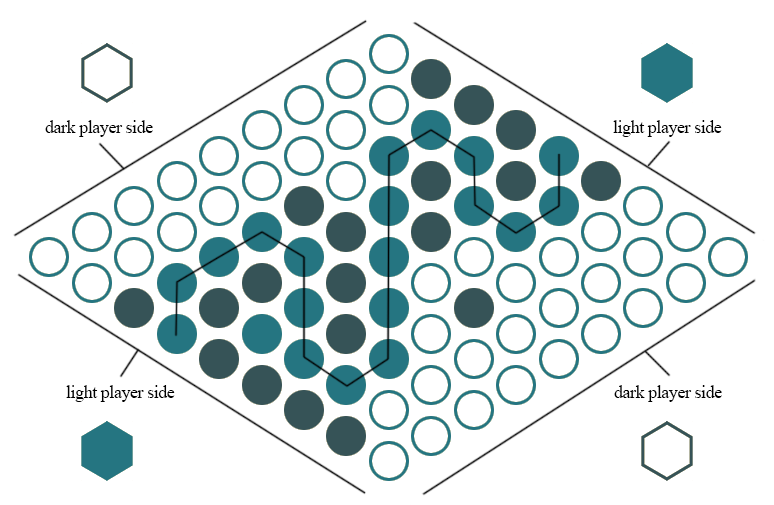
\includegraphics[width=0.7\textwidth]{figures/hex-winning}
	\caption{A 9x9 game where the light blue agent has won, as its two sides, the left to bottom and the top to right, are connected. The connection is illustrated with a line, showing the unbroken connection between the two sides.}
	\label{fig-winning}
\end{figure}

With the above-described rules, the first player has a strong advantage. As such, it is not uncommon to employ a \textit{swap rule}, where the second player, after the first player's initial action, has the option to swap and become the first player and transpose the position of the piece. This evens out the first player advantage. However, since I intend to keep the game part of the project as simple as possible, I will ignore the swap rule.

\subsection{Complexity}
Because of the similarity of the rules of Hex and Go, in terms of how the board is configured and their turn based nature, it also exhibits a similar game complexity, when equal board sizes are used. Complexity specifically in the form of a rather high branching factor.

An advantage of Hex is that the simple rules allows for a simpler software implementation of the game, and said rules allows for adjustment the complexity by either decreasing or increasing the board size. 

Increasing the size of the board in Hex, similar to Go, is not trivial, when looking at how it affects the game tree complexity. If one estimates an average Hex game length to be $40\%$ the number of board positions, that would amount to $\approx 32$ for a 9x9 board, and $\approx 20$ for a 7x7 board. The average branching factor would then be $81 - 32 / 2 = 65$ and $49 - 20 / 2 = 39$ respectively. We can then roughly estimate a lower bound of the game tree complexity, as the average branching factor to the power of the average game length: $65^{32}\approx 1.03 \times 10^{58}$ for 9x9, and $39^{20} \approx 6.63 \times 10^{31}$ for 7x7. A quite significant increase.

\subsection{Strategies and AI agents}
An early Hex playing AI agent was constructed by Claude Shannon and Edward F. Moore, and described by the former in a paper in 1953. To put it in the author's own words, it was among the type of \textit{"Machines applying general principles of approximate validity"}\cite[705-706]{Shannon1953}. Their agent was interestingly built as an analog device, that functioned as a resistance network, with electrical resistors as edges and light bulbs as positions. One player's pieces had positive charges, the other negative. This device proved to play pretty well against humans, especially when it was the starting player. It did suffer from being unable to come up with reasonably good end-game combinatorial plays\cite{Shannon1953}.

The winner of the 5th Computer Olympiad in 2000, in Hex, was Hexy, an agent created by Vadim V. Anshelevich. It uses an evaluation function similar to Shannon and Moore's device, but enhanced by a theorem proving algorithm that finds virtual connections. Virtual connections, as opposed to realized connections, are board subpatterns, where one player is guaranteed to be able to create a connection, no matter how the opposing player plays in that subarea, given they play optimal\citep{Anshelevich2000}.

An illustration of 3 simple virtual connections, known as two-bridges, can be seen in figure \ref{fig-two-bridge}. Even though it is the dark player's turn, it can not prevent the light player from connecting its two sides, if the light player plays optimally. Each of the letter-marked position pairs \textbf{ab}, \textbf{cd}, and \textbf{ef} performs a two-bridge, where if the dark player places a piece in one of the positions, the light player can place a piece in the corresponding position of the pair. It should be noted that Hexy also looked at more advanced virtual connections, and that the evaluation function was applied in a alpha-beta search algorithm.

\begin{figure}[ht]
	\centering
	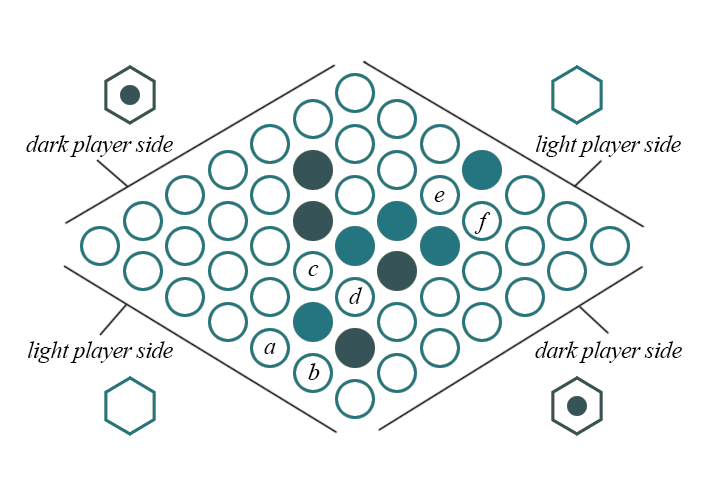
\includegraphics[width=0.6\textwidth]{figures/hex-two-bridges}
	\caption{Illustration of 3 \textbf{two-bridges}.}
	\label{fig-two-bridge}
\end{figure}

Among the most successful newer Hex-playing agents have been MoHex and MoHex 2. MoHex, among other approaches, combines Hexy's method of evaluating virtual connections with MCTS. MoHex 2 is a further extension of MoHex, where the MCTS search is further aided by  a supervised machine learning algorithm that is trained on win correlation of board patterns. In the paper describing MoHex 2, the creators interestingly state that according to their findings, an algorithm with only MCTS and some other features, but missing the explicit virtual connections evaluation, borrowed from Hexy, perform rather badly. They suggest that their MCTS simulation policy is unable to observe global virtual connectivity\cite{Huang2014}.

A final Hex playing agent I want to mention is EXIT\cite{AnthonyThomasandTianZhengandBarber2017}. Like AlphaZero it also uses a reinforcement learning neural network, starting from tabula rasa knowledge. However, it is closer to AlphaGo Zero, in that it employs separate neural networks for value and policies. The EXIT algorithm were able to beat MoHex on some different settings\citep{AnthonyThomasandTianZhengandBarber2017}.

\section{Validating performance}
To find out if the trained agents have actually learned anything, some game-playing performance measuring is necessary. A very simple way of doing so is to measure win rate against a baseline agent. For this I intend to use a simple non-neural network MCTS implementation, playing with a significant amount of simulations.

Another more complicated way is to measure some sort of Elo rating among the agents, as they play against each other. To be able to answer the question of whether my learned agents are able to acquire a state-of-the-art playing skill, I think including other agents than the baseline MCTS is required. Therefore I intend to use Hexy, on expert settings, against the most promising of the experiments from this project, in addtition to the baseline MCTS. I would also have liked to include newer developed Hex playing agents, like MoHex 2 and EXIT, but were not able to find runnable versions of them.

To estimate ratings, I intend to use a freeware tool by French computer scientist Remi Coulom, that estimates Bayesian Elo ratings\cite{Coulom}. Bayesian Elo rating, which in difference to more regular Elo ratings, takes uncertainty, in regards to sample size, into account, and the specific implementation also takes information about which player is first, into account. Even though the program is originally developed for Chess games, I think it is suitable for the task.

\section{Recapitulation}
To sum up the background and analysis chapter, I will return to my adaptation of Tom Mitchells machine learning definition, and now elaborate on each of the three parts.

The task \textit{T} at hand is still to play the game of chess. But considering that DeepMind spent what is equivalent to 178 years of TPU time while generating 19x19 Go game data, I find it reasonable that I, with my single RTX 2060 available, scale the Hex boards, I will train models on, down. Additionally, for the sake of simplicity of the implementation, I will also ignore the swap rule. How the algorithm executes the task will be inspired by the AlphaZero approach that makes use of both a Residual Neural Network for value-policy inference, and a Monte Carlo tree search that looks for good moves, in accordance with what the network returns.

The performance \textit{P} will be measured against other trained models, as well as a baseline MCTS agent. However, since pure MCTS is not that good at playing Hex, as stated in the Mohex 2 paper\cite{Huang2014}, I will also use Hexy to match up against.

The experience \textit{E} will be generated through self-play, and starting from tabula rasa. In addition to a scaled down board size, I don't expect to be able to generate the same amount of games that DeepMind has been able to. Again, because I have to take the smaller amount of computational power available to me into consideration, it is interesting to use the Tensor cores that the RTX 2060 provides, which will require network models that use half-precision floats. This should allow me to speed up the process of generating game data, and as such more data to train on should be available.